% Chapter Template

\chapter{Dataset Used: MAHNOB-HCI Tagging Database} % Main chapter title

\label{Chapter4} % Change X to a consecutive number; for referencing this chapter elsewhere, use \ref{ChapterX}

\lhead{Chapter 4. \emph{Dataset Used: MAHNOB-HCI Tagging Database}} % Change X to a consecutive number; this is for the header on each page - perhaps a shortened title

The components of the database are as shown in the diagram below.

\begin{figure}[H]
\centering
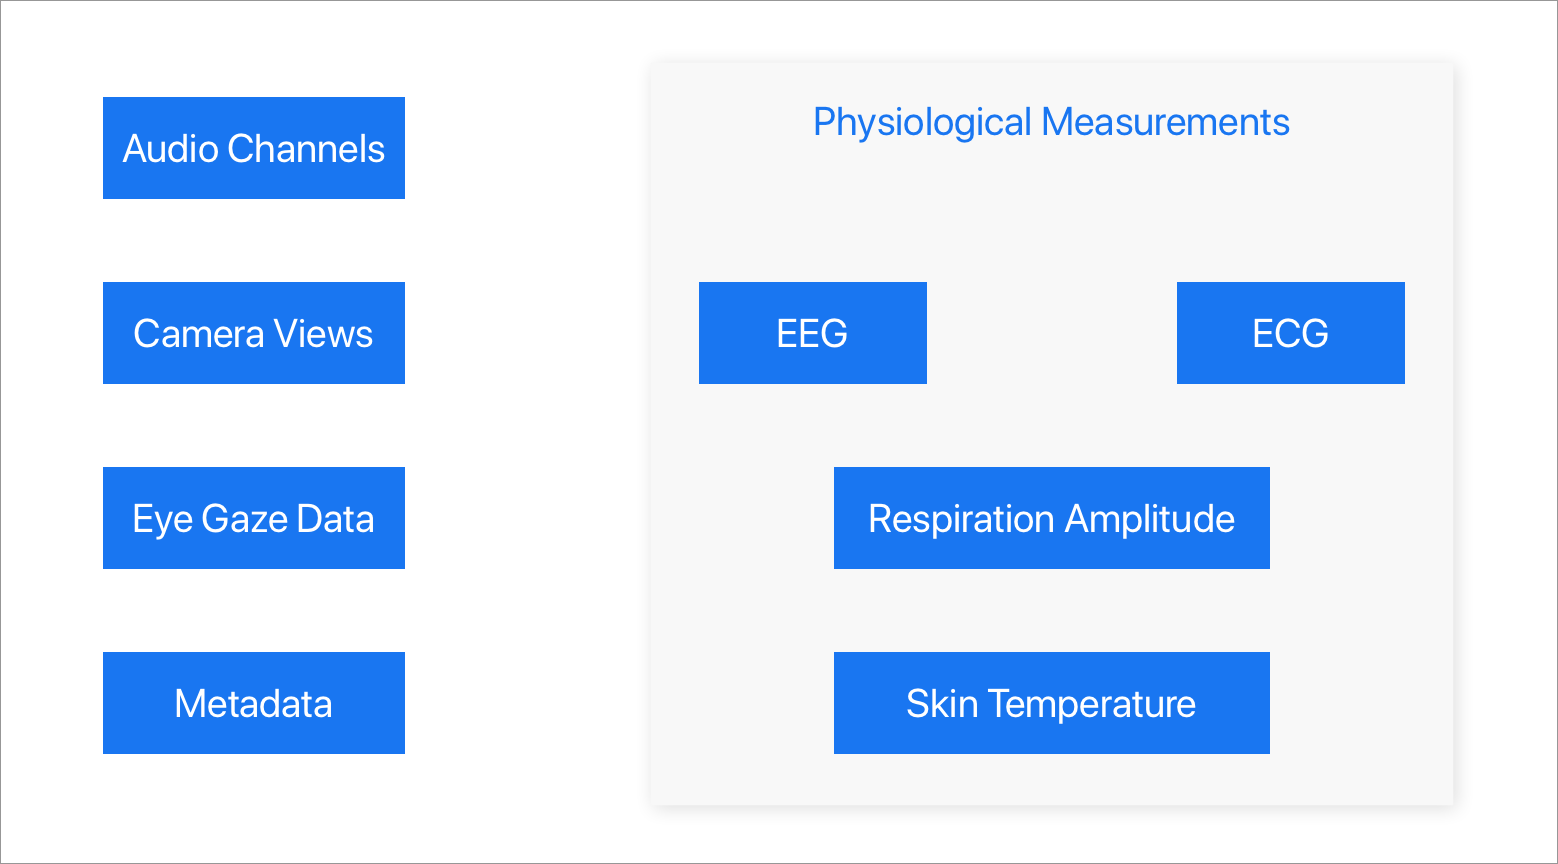
\includegraphics[height=7cm]{Figures/dataset.png}
\caption{MAHNOB HCI Components}
\label{fig21}
\end{figure}

The experiment data was collected from 30 healthy volunteers, comprising 13 male and 17 female between 19 to 40 years old. EEG Signals were recorded from 32 active electrodes on 10-20 international system using a Biosemi Active II system. A total of 546 emotion elicitation experiments were conducted. The 32 EEG channels of interest along with their indices are shown below.

\begin{figure}[H]
\centering
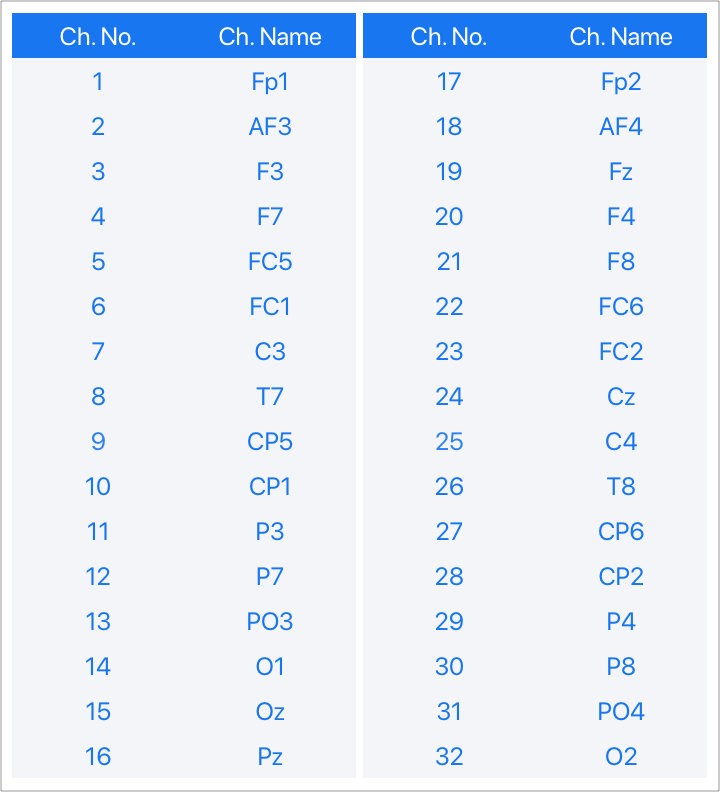
\includegraphics[height=9cm]{Figures/channels.png}
\caption{EEG Channels}
\label{fig22}
\end{figure}

Each Biosemi Data Format (BDF) file contains 47 channels out of which channels 1 - 32 are EEG signals, channels 33 - 46 are signals from other physiological activities, and channel 47 is the Status channel. The stimuli were videos included in the Hollywood Human Action dataset \cite{holly}. 20 videos were used in the experiment. Each subject watched all the 20 videos in a single run. So, in order to reduce the influence(bias) from watching the previous videos, the subject was shown neutral videos in between each stimulus video. Hence, in each BDF file, there is around 15 seconds of physiological readings of the subject both at the start and at the end of the emotion elicitation experiment. The exact point of time when the stimuli started and ended was marked in the Status channel, i.e., channel 47. The flow of the experiment with time is shown below.

\begin{figure}[H]
\centering
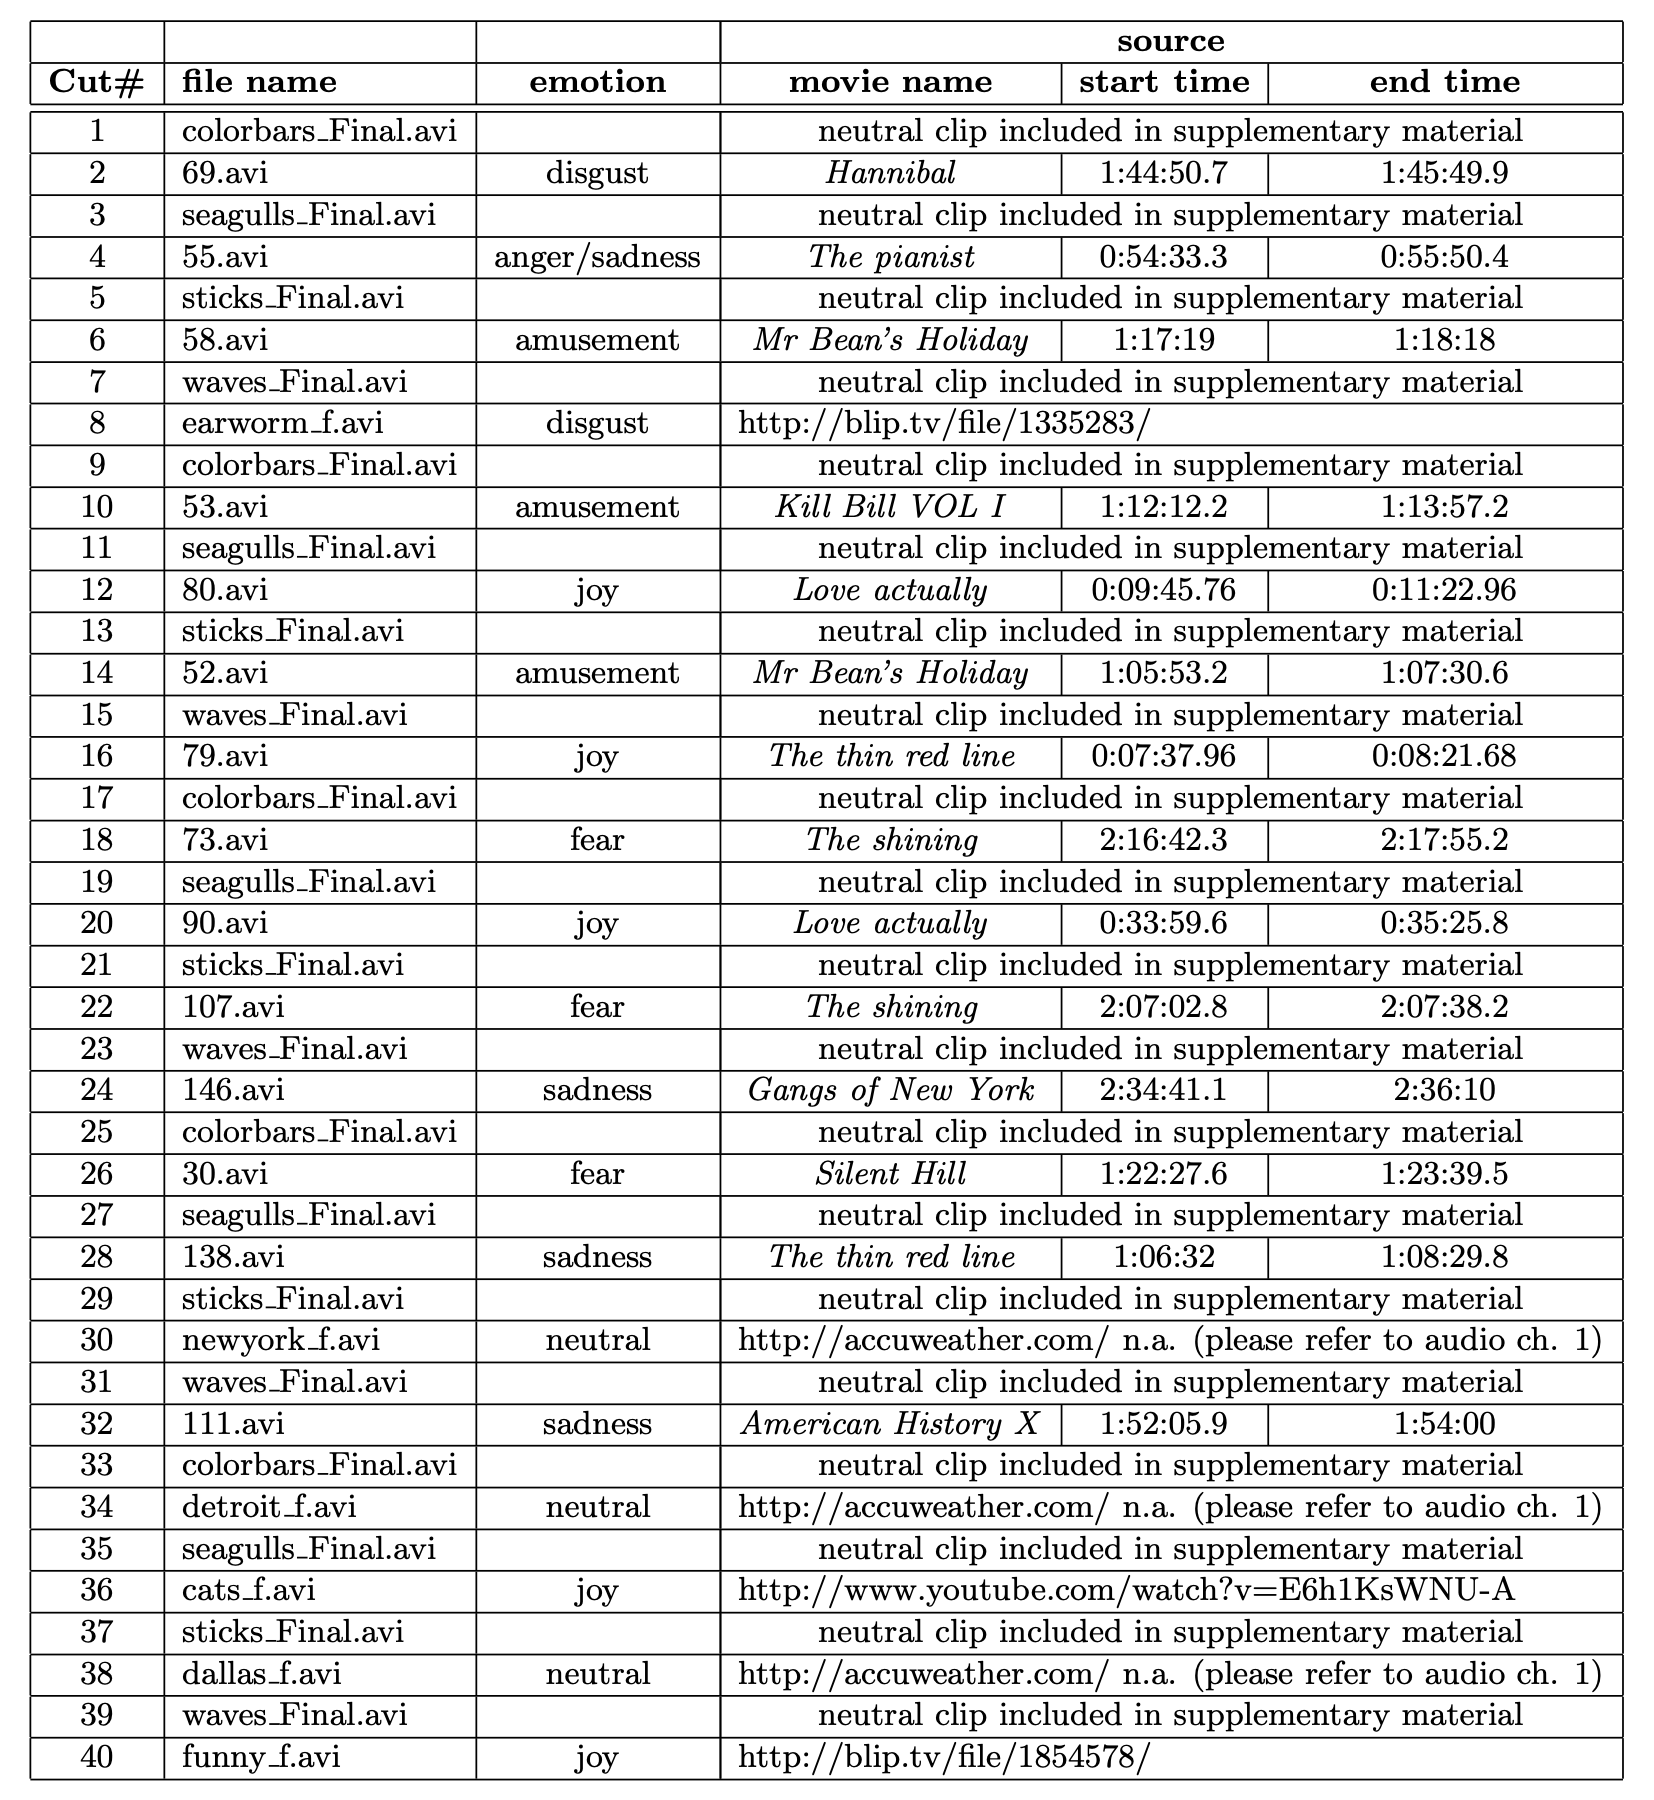
\includegraphics[height=17cm]{Figures/experiment_flow.png}
\caption{Experiment flow}
\label{fig22}
\end{figure}

The ground truth or labels for the emotion elicitation experiments consist of four orthogonal axes of measurement of emotion or affect:
\begin{enumerate}
    \item \textbf{Valence}: Valence is a psychological quality or quantity that depicts or measures, respectively, how attractive or averse the object of interest is perceived to be.
    \item \textbf{Arousal}: Arousal is a psychological measure that quantifies or qualifies how much stimulated the subject is. The psychological state of being awoken or active is measured by this value.
    \item \textbf{Control}: Control is a affective measurement that depicts how much control the subject has on his action and interpretation of events. ``People want their experiences to reflect the way that they see the world, so that the \textbf{does} of human behavior matches the \textbf{should} of human behavior as they see it.''(Affect Control Theory, Franklin College of Arts and Sciences, University of Georgia).
    \item \textbf{Prediction}: The predictability of the next events to occur by observing the events uptil now is measured using this scale.
\end{enumerate}
The labels in the dataset are integers in the range ${1, 2, \ldots 9}$, where 1 means the lowest and 9 means the highest values of that axis of measurement. 